% !TEX root = ../main.tex
%
\chapter{The (end of the) monocentric city}
\label{chap:monocentric_introduction}


\begin{flushright}{\slshape    
Our progress is narrow;\\
it takes a vast world unchallenged and for granted.}  \\ \medskip
--- J. Robert Oppenheimer~\cite{Oppenheimer:1954}
\end{flushright}

The hypothesis that cities organise themselves around a single center of
activities---the Central Business District in the US---may well be one of the
strongest hypothesis in urban studies. Although no one seriously believes in its
validity any more, its influence is still creeping, often unnoticed, in many
empirical and theoretical works.  In order to deconstruct the monocentric model,
we first need to understand where it came from in the first place, for what
reason it was introduced and what evidence it was based on. In this chapter, we
present a historical perspective on the monocentric hypothesis: the context in
which it was introduced, and how it was gradually realised that cities had a
decentralised structure. We will end with a review of the emergence of the
notion of center and of the tools developed to measure their number.

\section{From monocentric, to polycentric and dispersed cities}
\label{sec:introduction}

Maybe the least assuming way to represent the density profiles in cities is
through cloropleth maps or 3-dimensional representation where the $x$ and $y$
coordinates correspond to the original coordinates projected on the plane, and
the $z$ coordinate to the density. The former approach can be traced back as far
as $1898$ with Meunot's \emph{Des agglom\'erations urbaines dans l'Europe
contemporaine}~\cite{Meunot:1898} who drew a large number of density maps of
large Europen cities, later followed by Jefferson in
$1909$~\cite{Jefferson:1909} who did the same for several cities in the US,
Europe and Australia. On Fig.~\ref{fig:density_3d} we use the latter approach to
represent density profiles for two metropolitan areas in the US: Minneapolis-St.
Paul and Houston. \\


\begin{figure}
    \centering
    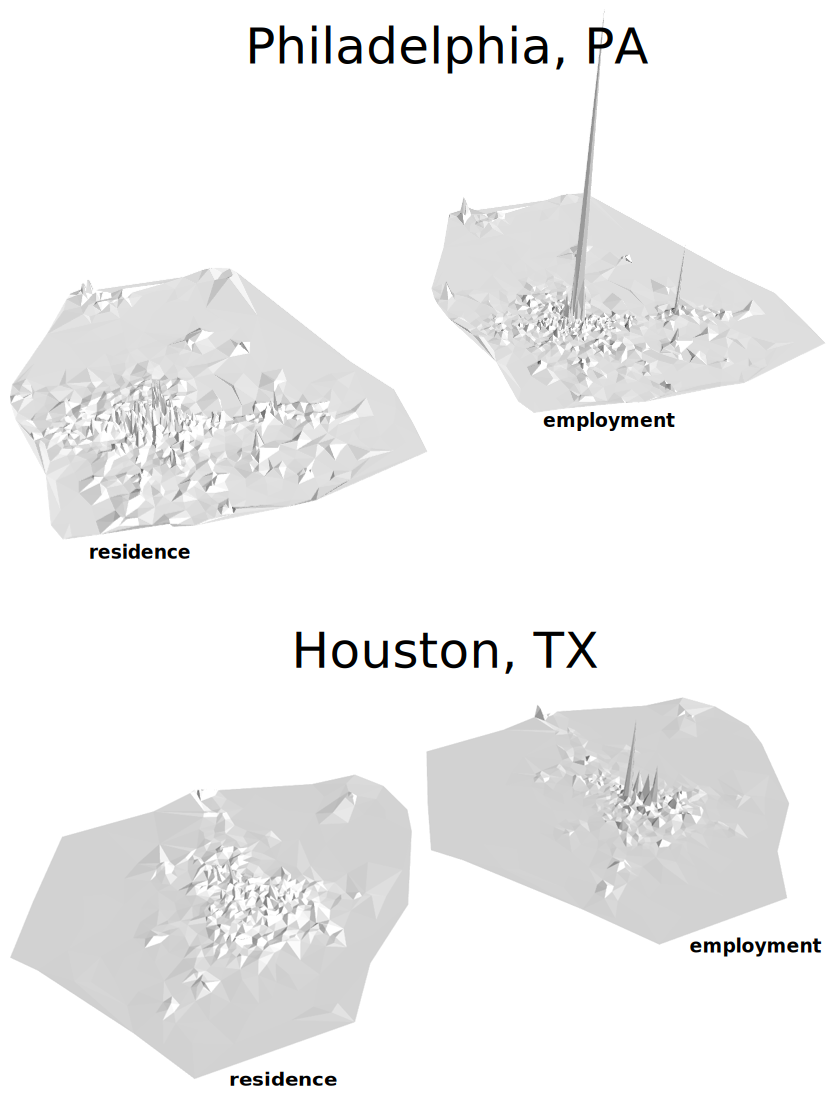
\includegraphics[width=\textwidth]{gfx/chapter-monocentric/panel_3d.png}
    \caption{{\bf 3D representations of densities.} (Top) The Metropolitan
        Statistical Area (MSA) of Philadelphia, PA. (Bottom) The MSA of Houston,
    TX. Employment and Population densities are plotted at the same scale.
Employment densities are sensibly more peaked than employment densities, making
the notion of `center' more intuitive. Data were obtained from the 2000 US
Census; the figures were prepared with Python and Inkscape.
\label{fig:density_3d}}
\end{figure}


These two cities are enough to get an idea of the difficulties associated with
studying density profiles.
First comes the question of what densities we are talking about. Indeed, people
are constantly moving throughout the city, and density profiles can only be
(approximate) snapshots of the city at different instants during the day.
Traditionally -- because of the availability of data -- people have mainly
considered the residence and employment density. This roughly gives an idea of
the densities in the city at night and during the day, and can thus help
understand the commuting patterns. We note that the availability of mobile phone
data that are continous in time might help to give a more precise, almost
real-time, and continuous picture of the densities during the
day~\cite{Louail:2014}.\\

Then comes the problem of how to makes sense of these patterns. The densities
represented on Fig.~\ref{fig:density_3d} are indeed very complex, and it would
help their understanding if we could isolate some particular structure.
This is what Clark did in $1951$~\cite{Clark:1951}. Realising that (1) districts of large
population tend to be in the interior, districts of small population in the
exterior (2) as cities expand, they tend to spread themselves out, he proposes
to write the density $\rho$ as a function of the distance $d$ from the center

\begin{equation}
    \rho = a\,e^{-d/b} 
\end{equation}

And, to justify his assumption, plots the population density of various cities as a function of
the distance to the center~\cite{Clark:1951}. The monocentric hypothesis was
born.

Looking at the density profiles plotted by Clark in 1951~\cite{Clark:1951} for
many cities across the world, or on Fig.~\ref{fig:distance_center_minneapolis}
for the Metropolitan Statistical Area of Minneapolis, one can be
forgiven for thinking that cities have a monocentric structure. Such profiles
indeed almost always exhibit a sharp decrease as we go farther from the city
center -- defined as the areal unit with the highest density. However, this
pattern is only the signature of a monocentric pattern if one makes the further
hypothesis that the pattern of employment densities in cites are symmetric
under rotations around the center. Obviously, this is not the case: cities are
nowhere isotropic but in the imagination of modelers. The decreasing exponential
model is thus mispecified.


\begin{figure}
    \centering
    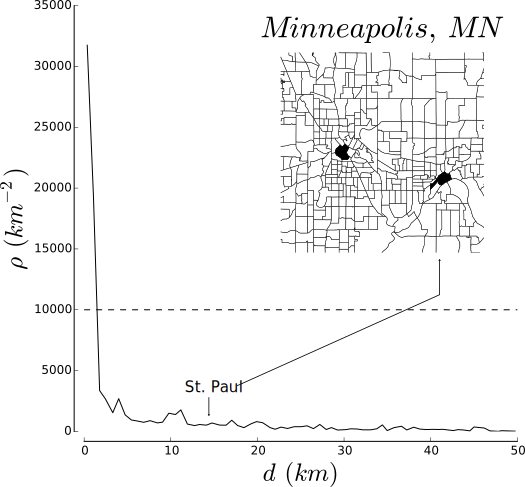
\includegraphics[width=\textwidth]{./gfx/chapter-monocentric/distance_center_minneapolis.pdf}
    \caption{Employment density as a function of distance to the center for the
    Metropolitan Statistical Area of Minneapolis-St. Paul in 2000. The center is defined here as the
    tract with the highest employment density, and corresponds to the historical
    Central Business District of Minneapolis. The curve exhibits a very sharp
    decay, giving the illusion of a monocentric structure. (Inset) The census tracts
    of Minneapolis-St. Paul in 2000. In black, the census tracts where the
    employment density reaches values above $10,000\,\text{km}^{-2}$. The two tracts
    coincide with the historical centers of the Twin Cities, and are distant from
    $14\,\text{km}$. This fragmented structure cannot be infered from the density
    profile on the left (arrow on the curve).
    \label{fig:distance_center_Minneapolis}}
\end{figure}


So why did Clark's methods and plots did not become a simple curiosity, but were
instead so widely adopted? Although we cannot explain why such and such and
things happened, there is little doubt that the echo this idea had in urban
economics has something to do with it. From an implied assumption in an
empirical analyis, the monocentric hypothesis only became clearly stated with
the theoretical work of economists.


The Alonso-Muth-Mills model (inspired by Von Th\"unen's land rent model)  might well be the reason for the long-lasting influence of
the monocentric model; a concise exposition of the model can be found
in~\cite{Brueckner:1987,Fujita:1989}). In 1964, Alonso introduced the bid-rent curve as a
function of the distance to the city center~\cite{Alonso:1964}. The simplifying hypothesis of
\emph{monocentricity} naturally followed, the assumption that all firms in a
city are concentrated in a single, fixed-size part of the city, the central business
district. Later, in $1967$ and $1969$, Mills~\cite{Mills:1967} and
Muth~\cite{Muth:1969} show how we can can obtain an exponentially decreasing
function for the density as a function of the distance from the center, using
the monocentric hypothesis. The monocentric Alonso-Muth-Mills (AMM) model was
born, and was seemingly backed by empirical evidence.\\


We should not underestimate how this model influenced people's perception
of what a city is. In the US, the name of Central Business District is casually
used as a way to designate the principle activity center in a city.  Many, if
not most, measures of the spatial variation of quantities inside cities actually
use the notion of `distance to the city center'. This biais can still be found
in the recent literature. For instance in a recent study by Glaeser, Kahn and
Rappaport on the repartition of income classes in cities~\cite{Glaeser:2008},
the authors comment on plots of the average income as a function of the distance
to the center. This only makes sense, however, under the assumption of monocentricity.
In fact, measuring quantities as a function of the distance to the center is
omnipresent in the literature. Many authors are relying on the monocentric
hypothesis for their empirical analysis -- sometimes without being aware of
it.\\

This persistence of the monocentric hypothesis is all the more surprising that
authors repeatedly suggested or found that the hypothesis was not adequate. In
other words, that the monocentric model that has dominated the field of urban
economics for now more than 4 decades, bears little resemblance with the
empirical reality. In
$1974$, Kemper and Schmenner~\cite{Kemper:1974} explore of industry and
employment density, trying to fit a negative exponential function. Their
conclusion is clear: ``A declining exponential function fails to explain much of
the spatial variation of manufacturing density''. Later,
Odland~\cite{Odland:1978} explores the possibility of polycentric cities on a
theoretical basis. As explained in~\cite{Griffith:1981}, people then started to
explore the density patterns of cities by fitting multi-center exponential
functions of the form

\begin{equation}
    \rho_i = \sum_{j=1}^{q} A_j\,e^{-d_{ij}/b_j}
    \label{eq:multi-exponential}
\end{equation}

where $\rho_i$ is the density at location $i$, $q$ the number of centers and
$d_{ij}$ the distance between locations $i$ and $j$. The idea of polycentricity,
originally as the generalisation of the monocentric hypothesis, is progressively
gaining ground. 

Trying to fit equations like Eq.~\ref{eq:multi-exponential} is
cumbersome, and requires some a-priori knowledge of the density patterns. It
requires to determine in advance which parts of the cities are going to be
subcenters \graffito{{\bf sub}center because they are subsidiary to the
traditional CBD}, before tring to fit the density profile. As noted
in~\cite{Giuliano:1991}, many authors used completely arbitrary definitions of
subcenters, either designating them based on their own intuition, or refering to
the centers defined by planning agencies. 

In this context, the first definitions of employment centers independent from
the exponential model start to emerge, and subcenters start an existence of
their own (see following section for an historical perspective on the measures
of the number of centers). By the $90$s, the idea that cities can be
polycentric well-established, and more and more empirical analyses confirm the
existence of several employment centers.  For instance, \cite{Dokmeci:1994}
shows that Istanbul's employment is spread across several centers. The centers
are not necessarily `subcenters' in the sense that activities do not necessarily
accumulate in the traditional downtown.  Indeed, Garreau~\cite{Garreau:1991}
introduces the concept of `Edge cities', the concentration of business, shopping
and entertainment can also occur at the outskirts of cities, in regions that
were previously rural, or residential.\\

\section{How to measure polycentrity}
\label{sec:how_to_measure_polycentrity}

\subsection{Urban form (put somewhere else)}
\label{sub:urban_form_put_somewhere_else_}

The methods to identify the employment subcenters can be roughly divided in
three categories: clustering methods, regression-based methods and distribution
based methods. The former
historically appeared first, and were progressively abandonned for the latter
due to the use of arbitrary cut-offs. But they made a come-back recently with
the developement of non-parametric clustering methods.\\

\subsubsection{Clustering methods}
\label{ssub:clustering_methods}


In $1987$, McDonald~\cite{McDonald:1987} remarks that despite being mentionned
in the empirical and theoretical literature, none discusses the features that an
employment subcenter should have. For the first time, he proposes a method to
determine the number of subcenters empirically. In fact he proposes to different
definitions, based on employment density and the employment-to-population ratio. Given
a number $T$ of areal units, we will say that $i$ with employment $E_i$,
population $P_i$ and surface area $A_i$ is an employment subcenter if:

\begin{itemize}
    \item The gross employment density $\rho_i = E_i/L_i$ is greater than that
        of the contiguous units;
    \item OR if the employment-to-population ratio $E_i/P_i$ is greater than
        that of the contiguous units.
\end{itemize}


Giuliano and Small~\cite{Giuliano:1991} acknowledge the necessity to
consider employment densities to define subcenters put forward by
McDonald~\cite{McDonald:1987}. However, they deplore that the method does not
allow for adjacent units with a high employment density to be centers -- as only
the larger one would be selected. Thus, they propose that we should say that a
continuous set of zones $\mathcal{S}$ is a subcenter if 

\begin{itemize}
    \item The employment density $\rho$ in that set is greater than a threshold
        $\overline{D}$;
    \item and the total employment $E$ contained in this set of units is greater than a threshold
        $\overline{E}$.
\end{itemize}

where the thresholds $\overline{D}$ and $\overline{E}$ are imposed arbitrarily.
Using this definition, all areal units with a high employment densities are part
of a subcenter, unless they are small (contain less than $\overline{E}$
employees), or isolated (i.e. they do not belong to a cluster containing at
least $\overline{E}$ employees).
As mentioned in~\cite{Anas:1998}, because density landscapes are highly
irregular at fine-scale (look at Fig.~\ref{fig:density_3d} for instance), the
subcenter boundaries are however very sensitive to the threshold values. Because
there are no a priori reason to choose a threshold rather than another, the
obtained subcenter boundaries are thus completely arbitrary, and are likely to vary from one
author to another. In other words, these methods lack a proper consideration,
based on first-principles, of how large is `large' supposed to mean.

Furthermore, the number of centers depends on the size of the areal unit, an
issue that is tied to scale problem discussed in the Modifiable Areal Unit
Problem (MAUP)~\cite{Openshaw:1986} literature. Indeed, small areal units will
lead to several low employment density units in otherwise very high density
areas. On the other hand, large areal units are likely to smooth over local
employment peaks. This begs the question of how to define `continuous' set, and
whether we should use contiguity, or rather proximity.\\


\subsubsection{Regression-based methods}
\label{ssub:regression_based_methods}

To adress these concerns, McMillen~\cite{McMillen:2001} proposes a two stage
procedure. In the first, non-parametric stage, the method consists in using a
geographically weighted regression (GRW, see~\cite{Brunsdon:1998} for more details on
the topic) to `smooth' the employment density, using distance rather
than contiguity as a measure of proximity, thus partially solving the issue
linked with the size of areal units--although not totally, since a span needs to
be determined to perform the GWR. Candidate subcenters are the units that
have unusually high employment densities compared to the broad spatial trends.
If we note $\rho_i$ the employment density at site $i$, $\hat{\rho}_i$ the
density estimated with GWR and $\hat{\sigma}_i$ the standard deviation around
this estimate, $i$ is said to be a \emph{candidate} subcenter if 

\begin{equation}
    \rho_i - \hat{\rho}_i > 1.96\,\hat{\sigma}_i
\end{equation}

Candidate, because the GWR only identifies fluctuations in the density profile,
with no consideration of whether these local fluctuations have a sensible impact
on the employment density. A problem with this approach is that candidate
subcenters are outliers with respect to an average that uses half of the total
points, thus losing the local information about employment
density~\cite{Redfearn:2007}.
Identifying which of these candidates are actually
centers is the goal of the second, semi-parametric procedure. The major problem
of McMillen's method actually resides in this second procedure, which uses
arbitrary criteria (the first and second largest candidates are omitted in the
regression, candidates at less than $1$ mile from the CBD are omitted), and a
somewhat ad-hoc formula that takes the distance from the CBD into account to
produce the estimates to which real values are compared.

Redfearn proposes a non-parametric method that aims at correcting the issues
with McMillen's\cite{Redfearn:2007}. The estimation of the employment density is
done locally in order to keep intact the local structure of the density profile.
However, arbitrariness still lies in the choice of the span (the amount of data
that are considered to estimate the slopes at a given point).\\

\subsubsection{Distribution-based methods}
\label{ssub:distribution_based_methods}



The approach that we originally took in this thesis is radically different that
these regression-based methods~\cite{Louf:2013_polycentric}. We start with the
remark that one does not need to know the spatial arrangement of areal units
with different densities in order to know which ones are most important. Indeed,
local fluctuations that are registered as centers in the regression-based
methods are very likely to have a negligible contribution to the total
employment. Therefore, a good estimate of the number of centers should be given
by the shape of the employment density distribution alone. Because it does not
require any spatial knowledge, it makes the extraction of centers fairly easy
and fast, compared to the previous methods.\\


We start by building the rank plots of employment density $\rho$ inside the
areal units. These plots display a decay at least as fast as that of an
exponential. If they were an exact exponential, they could be modeled by a
function of the form

\begin{equation}
    \rho(r) = \rho_0\,e^{-r/r_c}
    \label{eq:}
\end{equation}

\begin{figure}
    \centering
    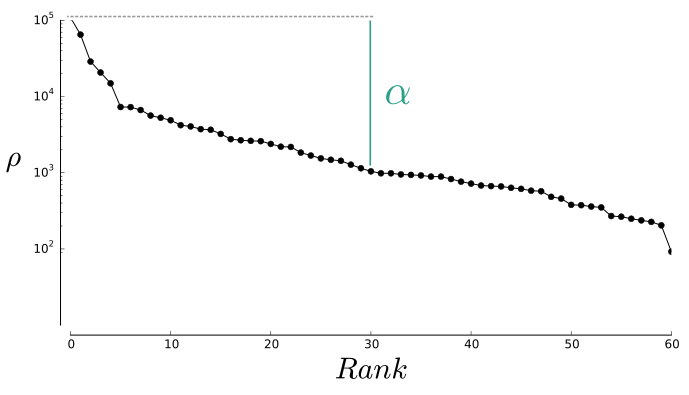
\includegraphics[width=1\textwidth]{gfx/chapter-monocentric/rank_plot_LA.pdf}
    \caption{Rank plot of the employment density in ZCTA's of Los Angeles, CA.
    \label{fig:rank_plot}}
\end{figure}

where $\rho(r)$ is the $r$th highest value of the density inside the city,
$\rho_0$ the maximum density value. This
exponential decrease implies that there exists a natural scale for the rank,
$r_c$, that we interpret here as the number of centers. In order to get the
number of centers, one would either need to compute the slope on a lin-log plot,
of find the value of $r^*$ for which

\begin{equation}
    \rho(r^*) = \frac{\rho_0}{e} 
\end{equation}

in which case $r^*=r_c$. However, the rank plots are not strictly exponential,
and we define the number of centers using a threshold value $\alpha$. We define
$\rho_m$ as 

\begin{equation}
    \rho_m = \frac{\rho_0}{\alpha}
\end{equation}

and the number of subcenters $k$ is equal to the number of values $\rho_c$ of
the density such that $\rho_c \in \left[ \rho_m, \rho_0 \right]$. In the case
where the rank plot would be strictly exponential, we would have

\begin{equation}
    k = \rho_0\,\ln \alpha
\end{equation}

so that the number of centers is mainly determined by $\rho_0$, small variations
in $\alpha$ should not change greatly the number $k$ of centers obtained.
The method however suffers from the need to use an arbitrary parameter, the
threshold $\alpha$ to extract the number of centers. As a result, we are not
sure to extract the `true' number of centers. Furthermore, it assumes a
particular form for the density distribution, which is likely to biais the
estimation.\\

In a subsequent article, Louail and Barthelemy~\cite{Louail:2014} propose a
generalisation of the previous method based on the Lorenz curve, often used in
Economics as a basis to quantify income inequality. Given the ordered set of
densities $\rho_1 < \rho_2 < \dots < \rho_T$ in the $T$ units, we plot the
proportion of cells $F=i/T$ as a function of the corresponding proportion of
employment density

\begin{equation}
    L_i = \frac{\sum_{n=1}^i \rho_n}{\sum_{n=1}^T \rho_n}
\end{equation}

so that both $F_i$ and $L_i$ take their values between $0$ and $1$. It is easy
to see that, in the case of a city with a uniform employment density, the
Lorentz curve is a straight line. In the general case, however, the curve has a
convex shape, with a more or less pronounced curvature.  The higher the
curvature of the Lorentz curve, the higher the inequality in terms of employment
density, and thus the smaller the number of potential centers. This lead the
authors to define a new criterion to determine the number of centers. It is
determined by the intersection $F^*$ between the tangent of the Lorentz curve at
the point $L(F) = 1$ and the axis $F=0$ (see Fig.~\ref{fig:loubar}. The units
that correspond to the values of $F$ between $F^*$ and $1$ are defined as
centers. This definition has the merit to only depend on the distribution of
density inside the areal units; it is genuinely non-parametric, while being
easily tractable and understandable.\\

\begin{figure}
    \centering
    \includegraphics[width=0.6\textwidth]{gfx/chapter-monocentric/loubar.pdf}
    \caption{An example of realistic Lorentz curve (solid black line), the curve
    that would be obtained in a city with uniformly distributed density (dashed
grey line), and the tangent at the point $L(F) = 1$ used to determine the number
of centers in the LouBar method.\label{fig:loubar}}
\end{figure}

Of course, all the methods presented here have their issues (see
chapter~\ref{chap:monocentric_discussion} for a discussion), and there is no
consensus on what method should be used to determine the employment centers.
There surely is more work to do before we arrive at a satisfactory picture of
urban form. Yet, the results given by these methods -- although slightly
different -- provide together a compelling evidence for the polycentric
structure of cities. 


\section{The polycentric transition}
\label{sec:the_polycentric_transition}

Mentionned occasionally in the empirical literature~\cite{McMillen:2007,
Readfearn:2007}, and hinted at in the urban economics models~\cite{Fujita:1982},
the greater polycentricity of larger cities was not firmly established before
this thesis. Almost all cities (apart from the notable exception of twin cities)
start growing around a single center of activity. Yet, as we will see, no large
city adopts a strict monocentric structure. Therefore, it seems that, as
they grow and expand, urban systems develop a more and more polycentric form. We
call this phenomenon the `polycentric transition' of cities. First, we will
gather the recent evidence for this polycentric transition. We will then review
the plausible explanations that can be found in the literature. This introduces
the next chapter where we present a model that explains the polycentric
transition of cities, while reproducing the empirical facts shown below. 

\subsection{Empirical evidence}
\label{sub:empirical_evidence}

Historical data over long periods of time, on a consistent set of areal units,
are very rare -- if not impossible to find. However, we do, for one point in
time, have many cities with very different population value. We can thus compute
and plot the number of centers as a function of population. Of course, as we
will discuss in more details in Part~\ref{part:scaling}, there is a gap between
evolution in time and transversal studies that is not completely obvious to
bridge.  Some cities can be, for historical reasons, locked into a monocentric
state where the average city would not. For different reasons, another city
might as well have developped a polycentric structure more prounounced than
other cities of the same size have. The idea here, is to look at a large number
of cities and measure the average behaviour of this ensemble of cities, hoping
that marginal cases are indeed marginal.


\subsubsection{American cities (census data)}
\label{ssub:american_cities_census_data_}

During this thesis~\cite{louf:2013_polycentric}, we used data on the employment in the Zip Codes of US cities
(which ones?) every year between 1994 and 2010. We first extracted the number of
centers for every city, for every year between 1994 and 2010. Using the
rank-plot method described earlier. We then applied the following treatment to
the data:

\begin{itemize}
    \item If there is only one Zip Code in the given city, $k=1$;
    \item We perform a Kolmogorov-Smirnov test~\cite{Massey:1951} between the
        distributions of a given city for consecutive years. If there is a
        significant difference (above a threshold $p_{KS}$) between the
        distribution at $t$ and $t+1$, we keep the point at $t+1$. If there is
        no sensible difference, we discard it.
\end{itemize}

At the end of this process, we obtain points that can be understood as coming
from different realisations of a city. We then plot the number of centers
obtained for all these realisations as a function of the total population and
obtain the curve obtained on Fig.~\ref{fig:us_centers}.

\begin{figure}
    \centering
    \includegraphics[width=0.9\textwidth]{gfx/chapter-monocentric/us_num-centers.pdf}
    \caption{Scatter plot for the estimated number of centers versus the
    population for about 9000 cities (different realisations) in the US. The red
dots represent the average population for a given number of subcenters. We fit
this average assuming a power-law dependence giving an exponent $\delta = 1.56
    \pm 0.15\,(R^2=0.87)$. Data were obtained from the U.S. Census Bureau's Zip
Code Business Patterns for every year between $1994$ and $2010$. The figure was
prepared with Python.\label{fig:us_centers}}
\end{figure}


A power-law fit on the average per population bin gives an exponent $\delta =
1.56 \pm 0.15\,(95\%\,C.I.)$. Thus, we find that on average, the number of
centers in US cities scales with population size as

\begin{equation}
    k_{\,US} \sim P^{\,0.64}
\end{equation}

\subsection{Spanish cities (mobile phone data)}
\label{sub:spanish_cities_mobile_phone_data_}

\begin{figure}
    \centering
    \includegraphics[width=\textwidth]{gfx/chapter-monocentric/spain_num-centers.pdf}
    \caption{Scaling of the number of centers with population for spanish
        metropolitan areas. Assuming a powerlaw relationship, the authors
    of~\cite{Louail:2014} find an exponent $\beta = 0.64$ ($r^2=0.93$). The data
were provided by Thomas Louail.\label{fig:centers_spain}}
\end{figure}

Using mobile phone data and the LouBar method to determine the number of
centers, Louail et al.~\cite{Louail:2014} also computed the number of centers
versus population for Spanish cities. Strikingly, the exponent they found is
very close to that we found on a different system of city, using a different
method to count centers, and a radically different data collection method.

\begin{equation}
    k_{\,Spain} \sim P^{\,0.64}
\end{equation}

The numerical values are, surprisingly, equal. Both studies agree on the fact that (1)
the larger cities are, the more polycentric they tend to be; (2) the average
behaviour is well-approximated by a power-law relationship between the number of
centers and population; (2) the increase of the number of centers with
population is \emph{sublinear}. This empirical regularity calls for an
explanation, and we will present in the next chapter a model that is able to
reproduce this empirical fact. But before concluding this chapter, let's have a
last look at the literature on urban form to see the reasons that are
traditionally involved for the polycentric transition.

\section{Reasons invoked for the polycentric transition}
\label{sec:reasons_invoked_for_the_polycentric_transition}

There are numerous examples where polycentrism finds its origin in the fusion of two
Metropolises, or the incorporation of satellite municipalities~\cite{LeNechet:2015}. For instance, the Twin Cities in the US, where the cities of
Minneapolis and St. Paul have grown to an extent where they now form a single
metropolitan area. The region of the Ruhr in Germany, or the region of Tokyo in
Japan are other examples. However, we are interested here in an endogeneous
polycentrism, caused by the growth of a single city.\\

Already in $1972$, Mills~\cite{Mills:1972}, suggests that congestion in large
metropolitan areas might be the cause of their decentralisation and
suburbanisation. However, we have to wait until $2003$ for McMillen to propose
an empirical study on the number of centers~\cite{McMillen:2003}. The author
finds a positive correlation between the number of centers and population, as
well as commuting cost. Commuting cost is estimated using the peak travel time
index index which is defined as the ration between the average travel time at
peak congestion time over the average travel time at any other time of the day.
Effectively, the commuting cost is a measure of the level of congestion in the
city. McMillen's empirical results on US cities show that there exists a strong
correlation between the number of subcenters in a city and its population and
levels of congestions. This implies that congestion might be the key factor to
understand the polycentric transition of cities.

\section{Summary}
\label{sec:summary}

In this chapter, we have presented an historical perspective on the monocentric
hypothesis, showed how it appeared, disappeared, and how it is still rampant in
most of the empirical literature. We then introduced the polycentric hypothesis,
how it was introduced, and the different methods that have been proposed to
measure the number of subcenters. We then showed empirically that larger cities exhibited a
more pronounced polycentric structure than smaller ones, and that the number of
centers versus the total population exhibited a regular behaviour, for many
countries and regardless of the data collection method or the method to count
the number of centers. This proves, we believe, the existence of a polycentric
transition of urban areas as their population increases. A transition which
might be due to increased levels of congestion.

In the next chapters, we will introduce a model that we developed during this
thesis in order to understand this polycentric transition. The model is able to
reproduce the variation of the number of centers with population, and we will
see that congestion alone is enough to explain this transition.

